\begin{figure*}[!t]
\begin{tabular}{@{}c@{}}
 	\begin{minipage}{42pc}
 		\centering
 		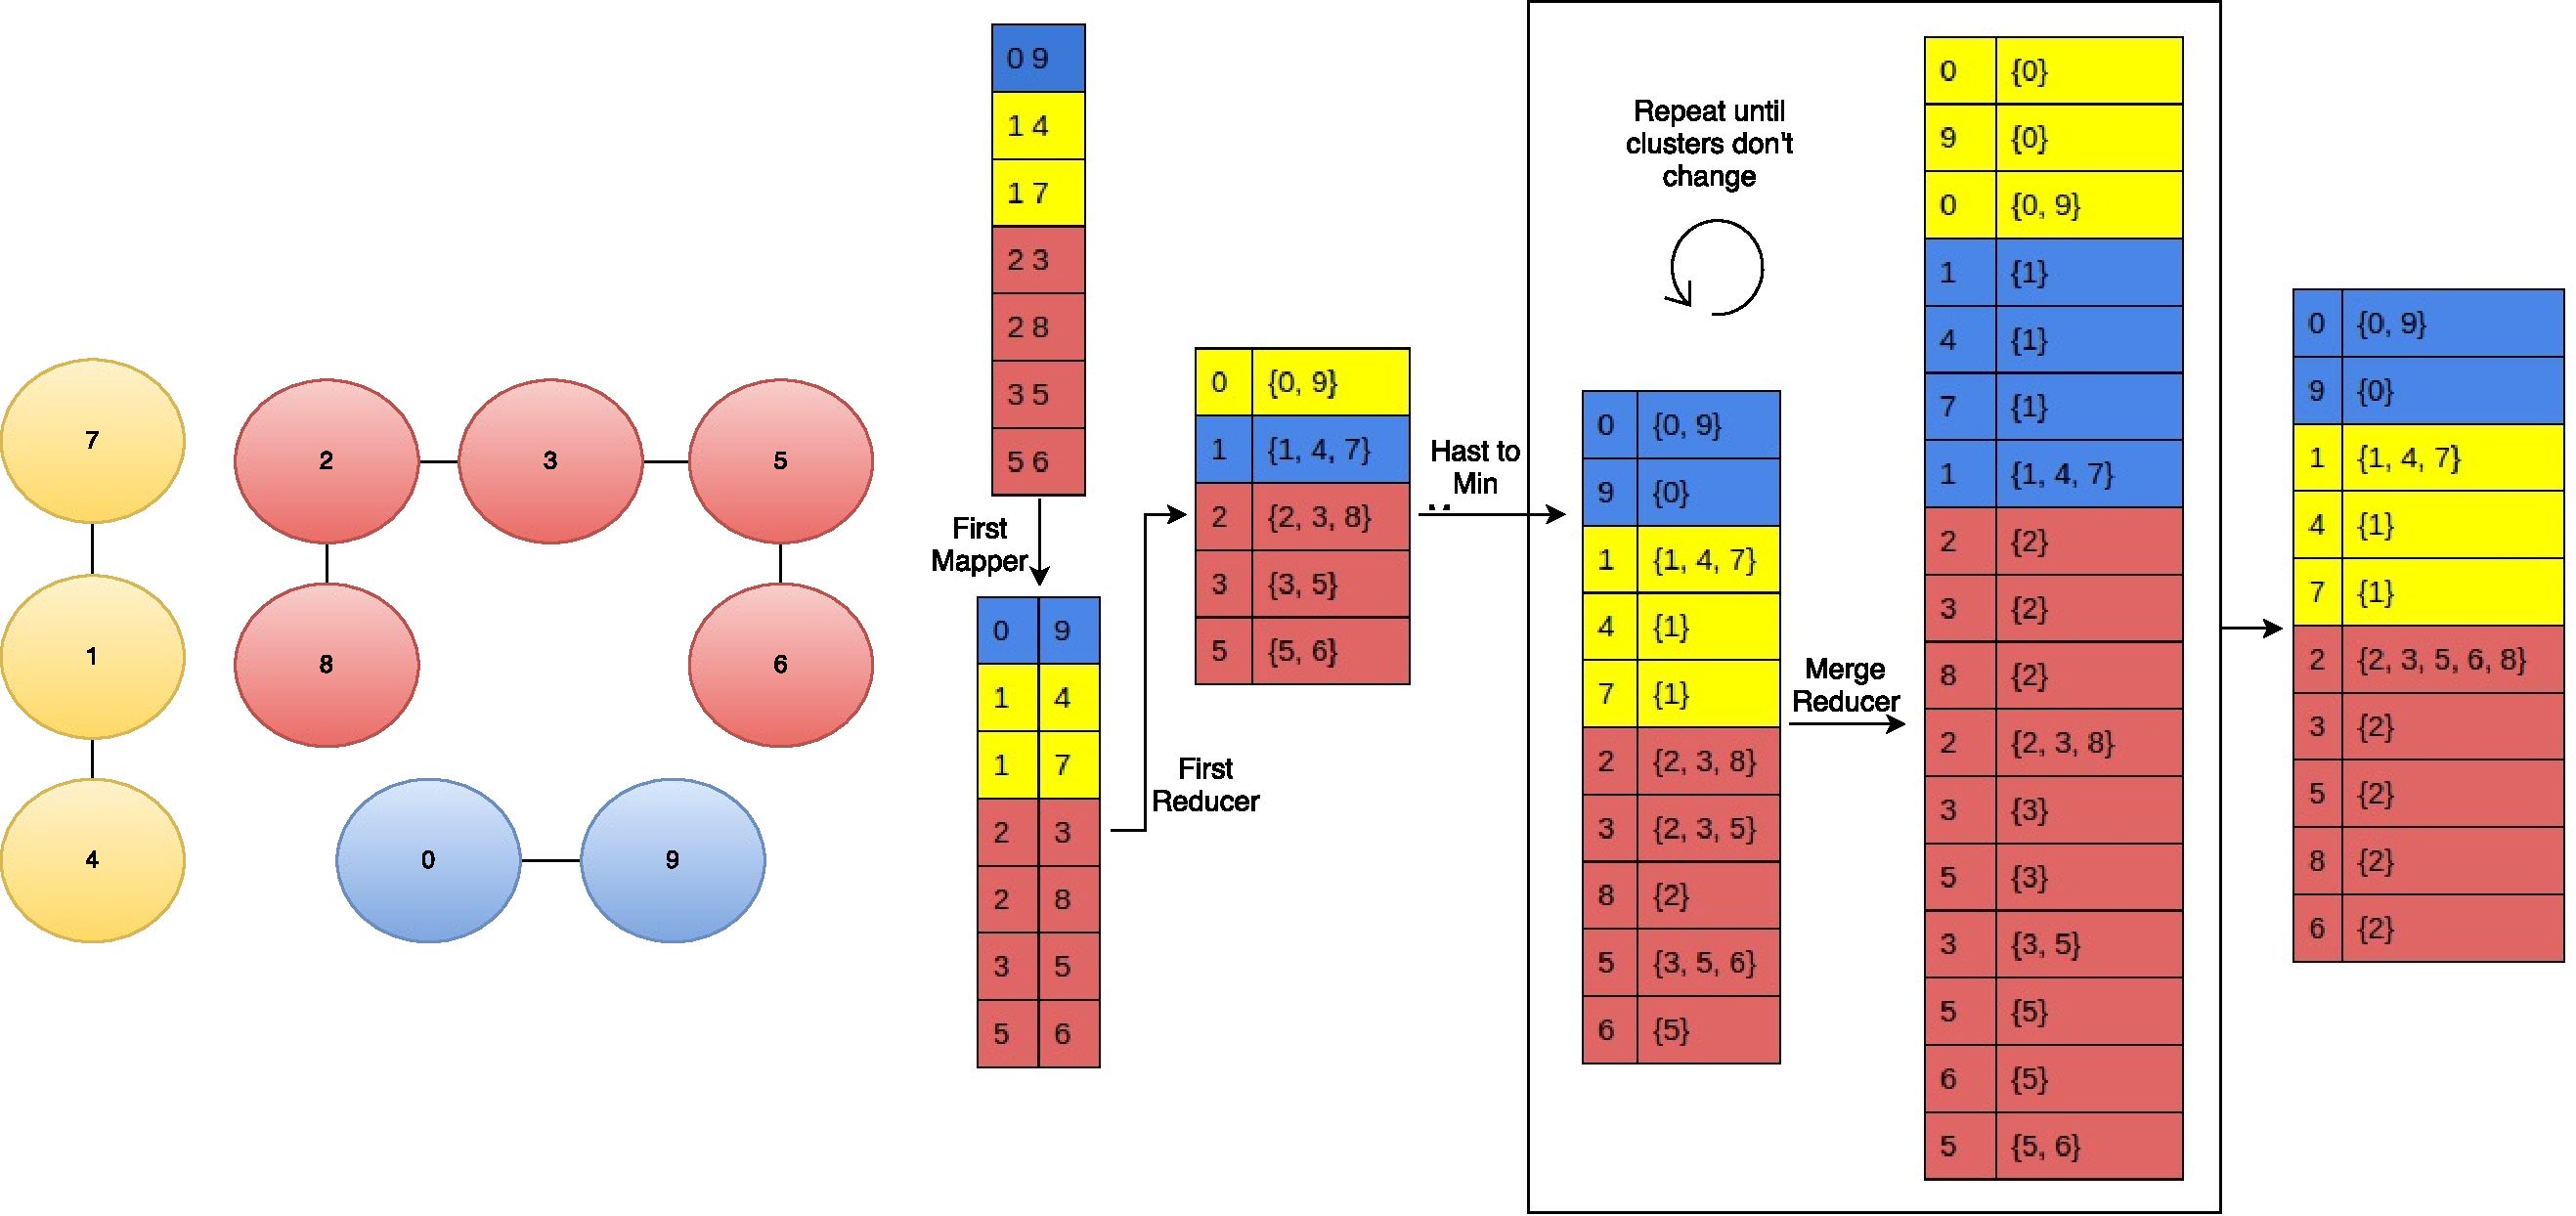
\includegraphics[width=40pc]{figures/mapreduce_example.pdf}
 		\caption{Example run of Hast-to-Min algorithm}
 		\label{figure:mapreduce_example}
	\end{minipage}
\end{tabular}
\end{figure*}

The analysis that follows for both the sequential and Map-Reduce parts assumes a graph G that can be formalized as $G=(V,E)$ where $V$ is the set of vertices in the graph labeled from $0 \to N-1$ where $N=|V|$ and $E$ is the edges set, which is a set of of 2-element subsets in $V$, that is $E \subseteq \{\{u,v\}: \in V\}$.

\subsection{Sequential}
A sequential algorithm of calculating connected components is used as a proof of concept to show the differences in performance when using Map-Reduce and compare when to use one approach over the other.

We chose to implement a variation of Tarjan's algorithm to find strongly connected components. Although this algorithm calculates strongly connected components in directed graphs, it can be used to find connected components in undirected graphs as well. Algorithm \ref{algo:tarjan} provides the pseudocode of our implementation. It is based on \cite{tarjan}. Essentially, it follows a Depth-First-Search (DFS) approach in exploring the graph and keeps track of the oldest ancestor it has found to associate as the leader of a connected component.

\begin{algorithm}
	\caption{Connected Components}
	\label{algo:tarjan}
	\begin{algorithmic}[1]
		\State Parse edges file
		\State Initialize graph as an adjacency list
		\State Initialize visited, stack, components
		\For {node $v \in nodes $}
			\If {$v \notin visited $}
				\State dfs($v$)
			\EndIf
		\EndFor
		\Function{dfs}{$v$}
			\State $visited[v] = true$
			\State $stack.push(v)$
			\State $isComponentRoot = true$
			\For {node $u \in neighbors(v)$}
				\If {$v \notin visited $}
					\State dfs($v$)
				\EndIf
				\If {$lowLink[u] > lowLink[v]$}
					\State $lowLink[u] = lowLink[v]$
					\State $isComponentRoot = false$
				\EndIf
			\EndFor
			\If {$isComponentRoot$}
				\State Construct component c from stack
				\State components.add(c)
			\EndIf
		\EndFunction
	\end{algorithmic}
\end{algorithm}

\begin{algorithm}[!h]
	\caption{Initialization Step}
	\label{algo:first_step}
	\begin{algorithmic}[1]
		\Function{Map}{$key, value$}
			\State $edge = value.split() $
			\State $emit(edge[0], edge[1])$
		\EndFunction
		\Function{Reduce}{$key, List<value>$}
			\State $outKey = new StringBuilder()$
			\For {$value \in List<value>$}
				\State $outKey.append(clusterSeparator).append(value)$
			\EndFor
			\State $emit(key, outKey)$
		\EndFunction
	\end{algorithmic}
\end{algorithm}

\begin{algorithm}[!h]
	\caption{Iterative Map-Reduce step}
	\label{algo:second_step}
	\begin{algorithmic}[1]
		\Function{Map}{$key, value$}
			\State $clusterNodes = parse(value)$
			\State $clusterNodes = cluster.split(clusterSeparator)$
			\State $v_{min} = min(node \in clusterNodes)$
			\For {$u \in clusterNodes$}
				\State $emit(u, v_{min})$
			\EndFor
			\State $emit(v_{min}, cluster)$
		\EndFunction
		\Function{Reduce}{$key, List<value>$}
			\State Initialize mergedCluster, maxSize
			\For {$C_v \in List<value>$}
				\State $elementsC_v = C_v.split(clusterSeparator)$
				\If {$elementsC_v.length > maxSize$}
					\State $maxSize = elementsC_v.length$ 
				\EndIf
				\State $mergedCluster.add(elementsC_v)$
			\EndFor
			\State $cluster = mergedCluster.toString()$
			\If {$maxSize < mergedCluster$}
				\State $context.counter++$
			\EndIf
			\State $emit(key, cluster)$
		\EndFunction
	\end{algorithmic}
\end{algorithm}

The algorithm's complexity is linear in the number of edges and nodes in the graph, \ie $O(|V| + |E|)$. This means that the algorithm will be very efficient for relatively small graphs, but it will start being ineffective while the graphs grow bigger and bigger up to hundreds of million vertices and edges. In particular, the parsing time of the input file would be the bottleneck since it has to be done sequentially as well as the available memory on the machine we are using, since the graph has to fit in its memory for Algorithm \ref{algo:tarjan} to work. Map-Reduce helps to eliminate exactly these restrictions, since the parsing can be performed in parallel in addition to running the actual connected components algorithm in a parallel fashion.

\subsection{Map-Reduce}

\subsubsection{Hash-to-min}


One of the algorithms that we chose for the Map-Reduce part is based on the Hash-to-Min algorithm introduced in \cite{rastogi}. This algorithm works in multiple logarithmic Map-Reduce rounds  to calculate the connected components of a graph at the end. In each round the algorithm merges overlapping clusters to compute connected components. Essentially, the algorithm can be imagined as a different Breadth-First-Search (\eg BFS) being performed in parallel. Each BFS builds up a connected component by combining smaller ones until there is convergence and the whole connected component has been discovered.

The are basically two phases in our Hash-to-min program for computing connected components. The first phase is the initialization phase which parses the input file and creates the graph as an adjacency list. The mapper emits a key-value pair for each edge in the graph and the reducer accumulates edges for each node and creates a mapping between nodes and list of neighbors. Algorithm \ref{algo:first_step} provides the pseudocode of this phase which is quite simple to follow.

Here comes the first optimization we performed in the original code using the Map-Reduce platform. The input file is processed in parallel using multiple mappers, thus utilizing the parallelism that we inherently get by running our program on Map-Reduce. For huge graphs, this phase should take less to complete than running on a single machine. It also overcomes any memory issues for storing the complete graph in memory on a single machine, since the graph is created in a distributed fashion by the reducers.

The second phase of Map-Reduce is the iterative step which merges together smaller connected components to form large ones in each iteration until convergence is achieved (\ie until there are no changes in the connected components calculated). Algorithm \ref{algo:second_step} shows the approach we follow in this Map-Reduce job. The map function calculates the minimum node in each cluster which we call $v_min$. Then it emits $(u, v_min)$ for each node $u$ in the cluster and also $(v_min, cluster)$. This aggregates the connected component to $v_min$ while reassuring that the rest of the nodes are associated with $v_min$ to avoid creating duplicate connected components. This is the second optimization in our approach. The alternative here would be to emit the cluster to each node (which leads us to a version of Hash-to-All algorithm in \cite{rastogi}), but that would only bloat the number of data being transmitted and add an additional overhead. Only one node is enough to represent the whole connected component and therefore an easy choice is to use the minimum labeled node as the component's representative. The reducer then takes all the clusters that are associated with one node and merges them together. If the final cluster has changed, we increment a counter to indicate this. If no more changes have taken place, the algorithm has converged. As shown in \cite{rastogi}, the algorithm will converge in $O(logn)$ steps, where $n$ is the total number of nodes in the graph.

The algorithm's complexity is linear in the number of edges and nodes in the graph, \ie $O(|V| + |E|)$. This means that the algorithm will be very efficient for relatively small graphs, but it will start being ineffective while the graphs grow bigger and bigger up to hundreds of million vertices and edges. In particular, the parsing time of the input file would be the bottleneck since it has to be done sequentially as well as the available memory on the machine we are using, since the graph has to fit in its memory for Algorithm \ref{algo:tarjan} to work. Map-Reduce helps to eliminate exactly these restrictions, since the parsing can be performed in parallel in addition to running the actual connected components algorithm in a parallel fashion.

\subsubsection{Two-Phase}

The other one we picked is based on the Two-Phase algorithm presented in \cite{kiveris}. It first introduces two operations over a graph and then how to combine them in order to to find the connected components.

Let $G = (V,E)$ and undirected graph, on $n = |V|$ nodes, and $m = |E|$ edges. For a node $v$, we denote by $\Gamma(v) = \{w|(v,w) \in E\}$ the neighbors of $v$ and $\Gamma^{+}(v) = \Gamma(v) \cup \{v\}$ as neighborhood of v and itself. Also, every node $v$ in the graph is associated with a real number label $l_{v}$. In the following we present the operations (small-star and large-star), which preserve the connectivity of the graph when performing them at all nodes in parallel.

\begin{algorithm}[!h]
        \caption{Small-star operation}
        \label{algo:small_star}
        \begin{algorithmic}[1]
                \Function{Map}{$u, v$}
                        \If {$l_{u} \leq l_{v}$}
                                \State $emit(u, v)$  
                        \Else
                                \State $emit(v, u)$  
                        \EndIf
                \EndFunction
                \Function{Reduce}{$u, N \subseteq \Gamma(u)$}
                        \State $m = u$
                        \For {$v \in N$}
                                \If {$l_v < l_m$}
                                        \State $m = v$
                                \EndIf
			\EndFor
                        \For {$v \in N$}
                                \State $emit(v, m)$
                        \EndFor
                \EndFunction
        \end{algorithmic}
\end{algorithm}


\begin{algorithm}[!h]
        \caption{Large-star operation}
        \label{algo:large_star}
        \begin{algorithmic}[1]
                \Function{Map}{$u, v$}
                        \State $emit(u, v)$
                        \State $emit(v, u)$
                \EndFunction
                \Function{Reduce}{$u, \Gamma(u)^{+}$}
                        \State $m = u$
                        \For {$v \in N$}
                                \If {$l_v < l_m$}
                                        \State $m = v$
                                \EndIf
                        \EndFor
                        \For {$v \in N$}
                                \If {$l_v > l_u$}
                                        \State $emit(v, m)$
                                \EndIf
                        \EndFor
                \EndFunction
        \end{algorithmic}
\end{algorithm}

\begin{figure}[ht]
  \centering
    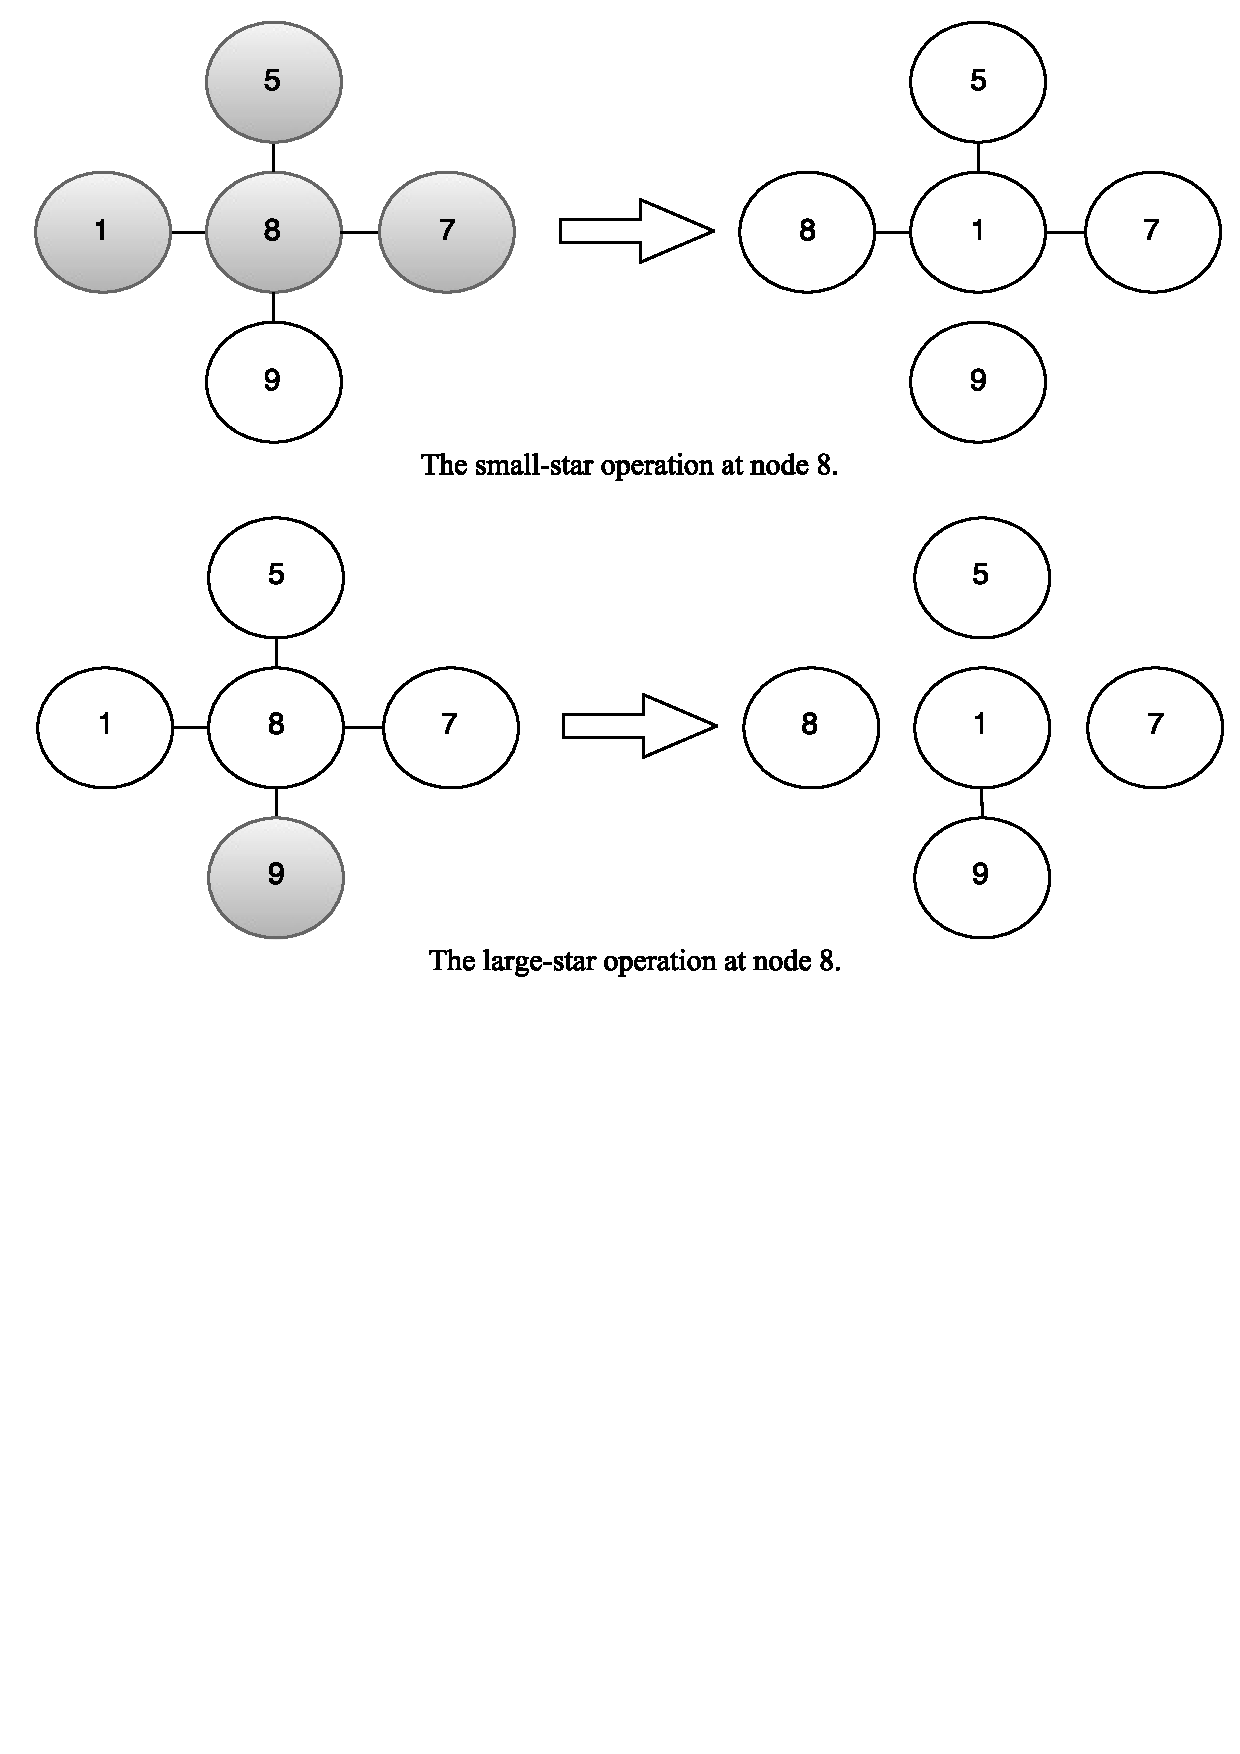
\includegraphics[width=20pc]{figures/two_phase}
  \caption{Small and large star operations}
  \label{fig:smalllargestar}
\end{figure}

These two operations can be combined and create the Two-Phase algorithm. In each inner loop, large-star is repeated until convergence is reached followed by one small-star operation. The outer loop is also repeated until convergence is met.

\begin{algorithm}[!h]
        \caption{Two-Phase Algorithm}
        \label{algo:two_phase}
        \begin{algorithmic}[1]
                \Function{Two Phase}{}
                        \Repeat
                                \Repeat
                                        \State $large-star$
                                \Until{Convergence}
                        \State $small-star$
                        \Until{Convergence}
                \EndFunction
        \end{algorithmic}
\end{algorithm}

Intuitively this algorithm efficiently simulates the classical Union-Find algorithm in parallel. In the inner-loop each node, finds its local minimum and adds an edge to it. In the outer loop, distinct local minimums are connected and then joined in a union step.

The Two-Phase Algorithm converges after $O(log^2 n)$ Map-Reduce rounds, which is higher than the Hash-to-min. The advantage it provides is a smaller communication size between consecutive rounds, making it able to handle bigger graphs in theory. This algorithm has proven to perform better than Hash-to-Min because of better load balancing in Map-Reduce rounds and sparsity of the transformed graphs.
